
\chapter{RobotME: Implementation}

\section{System Components}

As was outlined previously in the High-level Architecture section the main system components are:
Framework core itself, Enhancer, Log Server, XML Processor. There are no
separate components such as Recorder or Replayer (or more accurately: they are part of the
Framework core).

\subsection{Enhancer}
As was said in previous chapter, this component is a separate tool which gets an input Java archive (JAR) file
with the compiled Java mobile applications and returns `enhanced' the same Java archive
with the code related to the RobotME Testing Framework (specialized code is `injected' into original
JAR file). The Enhancer works in two modes: former represents recording/ capturing phase that creates
enhanced JAR with injected code that is able to intercept the user events;
and the latter represents replaying phase that creates enhanced JAR with injected code that
is able to simulate the previously captured events.

From the implementation point of view the Enhancer is a separate Java J2SE program, which is implemented as an ANT
task (so it can work as a stand-alone tool from the console and as part of the build process). The basic responsibility
of this tool is to investigate the compiled Java code of the input JAR file. The tool intercepts appropriate
parts of the code (in Aspect Oriented Programming these are called join points), modify them in expected way
and put back to the output JAR file.

The Java bytecode is a kind of assembler language with low-level opcodes. It is very difficult to investigate
such a code and find an appropriate places for interception. To do this the programmer
should feel comfortable with the great amount of different mnemonics of Java (There are between
200 and 256 mnemonics, depending on how the JVM has enhanced the standard
set with optimizing extensions). 
To simplify the work with bytecode there are various
aspect-oriented frameworks like AspectJ, AspectWerkz 
or even Spring Framework build-in AOP facility. Unfortunately these frameworks do not offer enough
expressive power to describe the injection points we mentioned earlier.
There is a finite set of transformations that AOP (aspect-oriented programming)
techniques can do (for example Spring Framework AOP mechanism creates only
proxies for classes it transforms; AspectJ can include various Java code inside Java methods,
but it also includes code strictly dependent to its own API which is not acceptable
-- mobile applications must be as small as possible). Due to all of these problems
we decided not to use the AOP frameworks at all. We concentrated on the Java bytecode modification
frameworks that offer not only more low-level access to the modifying bytecode but also offer
some help with transformations techniques. To our knowledge there are two most often
used open-source frameworks that fulfill such requirements: ASM and Apache
BCEL. Both of these frameworks were thoroughly
tested and verified. We have chosen ASM as a foundation for our Enhancer.
The choice was made because of:
\begin{itemize}
\item the company which supports ASM, France Telecom R\&D Center, guarantees good quality of the product;
\item ASM has substantially smaller memory and computation overhead compared to BCEL;
\item ASM is easier to use and covers both tree-like investigation of the Java bytecode as well as
  event-like (similarly to XML code parsing where these terms are called: DOM and SAX techniques respectively).
\end{itemize}

Having chosen bytecode modification framework we created base Enhancer architecture around the ASM
framework and its processing scheme which is based on visitor design pattern (event-like). The internal 
Enhancer's architecture is depicted on the class diagram on Figure~\ref{fig:uml-diagram-enhancer}.

\begin{figure}[t]%
\begin{center}
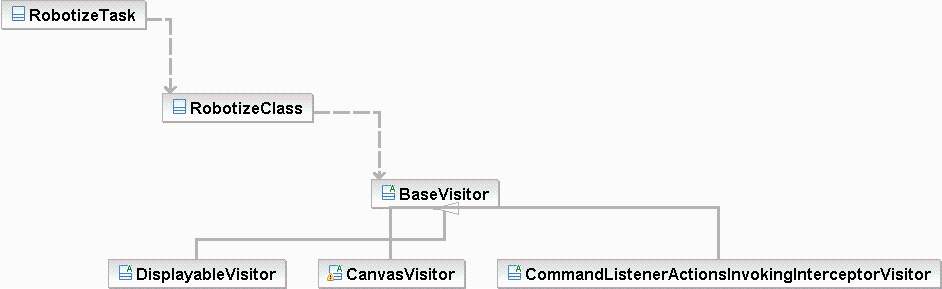
\includegraphics[width=\linewidth]{figures/uml-diagram-enhancer}
\end{center}
\caption{The implementation of Enhancer.}%
\label{fig:uml-diagram-enhancer}
\end{figure}

The presented classes are responsible for:

\begin{description}
    \item[RobotizeTask] it is the ANT task and entry point of the Enhancer tool. RobitizeTask has reference to the 
\code{RobotizeClass}.

    \item[RobotizeClass] is the main class responsible for delegating enhancing task to the appropriate utility components
 including: decompressing JAR file, iterating over Java class files, writing transformated bytecode to the
 Java class file, compressing back previously transformated code to the output JAR file.

    \item[BaseVisitor] each of transformation type is implemented in its own separate Java class and BaseVisitor
forms a base implementation for all of transformations and offer most frequently used methods like 
obtaining Java bytecode and managing lifecycle of the transformation process. It has many specific
implementations some of them are depicted on the diagram as classes that derives from it.
\end{description}

\subsection{Recorder}

The Recorder starts working when the mobile application (Midlet) begins execution inside
the KVM. The code injected into the original application calls internal classes 
of the RobotME core forwarding the required events. 

The main application's midlet is wrapped in the \texttt{RobotMERecorder} class. 
It is a singleton class and only one instance
of this class exists per one running mobile application. The framework is able to differentiate
between low-level events (key presses, pointer movements) and high-level events (commands invoked 
by the user). These events are passed to cooperating objects like: implementations of the \texttt{DisplayableState}
class and \texttt{LogHandler} and further to the Log Server component. 

There are cases when an event that occurred in the mobile application does not leave any changes
in the internal state of the mobile application. It is also \texttt{RobotMERecorder}'s responsibility
to detect such situations and react accordingly (log an intercepted event but with the
information that it is not candidate for the assertion verification because it leads
to no visible internal state changes).

\subsection{Replayer}

Replayer is an extended version of the recorder component (reason to such a case was mentioned in
the high-level architecture chapter). From the framework's internals point of view the Replayer is
really two cooperating things: one, a Java thread that constantly reads events from
repository (in current prototype implementation only files bundled into JAR file
are supported as repository). Based on a read event (\texttt{LogEntry}), this thread creates corresponding
\texttt{Replayable} object that knows how to replay a given \texttt{LogEntry}. The second
thing is \texttt{RobotMEReplaying} class. Reponsibility of this class is similar to
\texttt{RobotMERecorder} -- to intercept every event interesting from the RobotME Testing Framework
point of view and perform verification of the internal mobile application state.
If state of the mobile application violates those that was stored in the
application usage scenario assertion is triggered (assertions are further described
in Section~\ref{sect:assertionsandfailurenot}). If state of the mobile
application is as expected simulator runs without stopping itself.

\subsection{Log Server}

Log Server is another separate Java J2SE tool (similarly to the enhancer component). It works on desktop
machine and its responsibility is to constantly listening for the incoming events from the
mobile programs under test and then store each received event (not interpreting them). Log Server is 
internally dependent on the Framework Core component and uses some of its classes, mainly
as events encapsulations.

\begin{figure}[t]%
\begin{center}
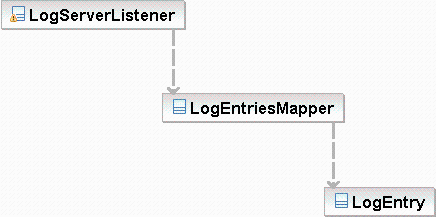
\includegraphics[width=.7\linewidth]{figures/uml-diagram-logserver}
\end{center}
\caption{Log Server implementation.}%
\label{fig:uml-diagram-logserver}
\end{figure}

Log Server architecture consists of one main class:
\texttt{LogServerListener}, that internally creates separate thread for each incoming
connections from the mobile application under test, therefor is able to receive
separate events from separate mobile applications, each connection not
interfere with any other (one connection per remote device).

\texttt{LogServerListener} is build in the way that it can be abstracted from the nature of
the underlying connection. It does not matter if the connection is performed as
a bluetooth or infra-red transfer, GPRS internet transfer or even simply
serial port connection (but what is usually important for the users is a price,
some of above connections are free of charge while the others might not be).
LogServerListener treat each connection type in the same manner -- as a form
of events transfer channel.

\texttt{LogEntriesMapper} -- is a class that knows how to create \texttt{LogEntry} class instance
from the received by \texttt{LogServerListener} event. Each \texttt{LogEntry} and also each event
are distinguishable by its unique ID number. To allow future implementations of
other special events (for example Nokia phones specific events) each ID
has its prefix and every internal events implemented as a part of the core RobotME Testing
Framework has its own reserved prefix. There is also a reserved prefix for custom,
third parties event IDs.

\subsection{XML Processor}

XML Processor is yet another separate Java J2SE tool. It is responsible for converting
stream of events (stored as a compact binary protocol) to the human-friendly
XML form of events. Its other task is to convert events back from human-friendly
XML form into compact binary protocol ready to replay on the mobile application.

Classes that take part in this processes are depicted on the following diagram.

\begin{figure}[t]%
\begin{center}
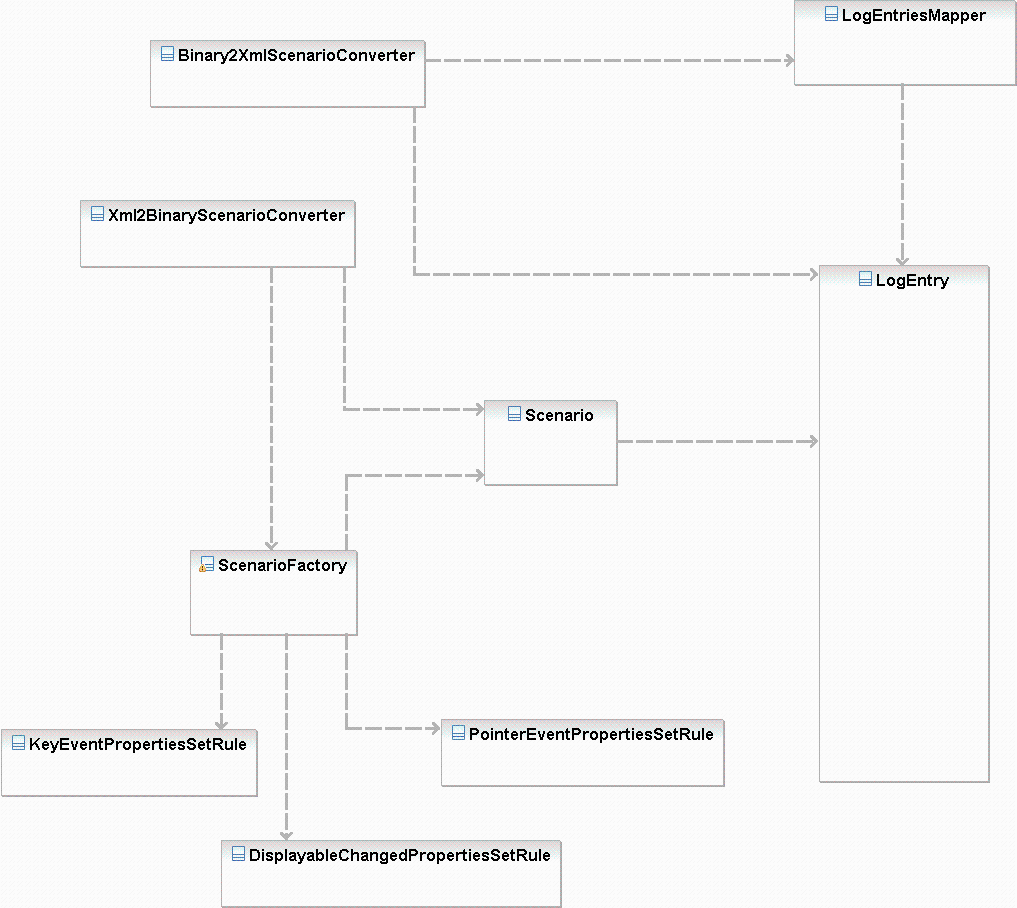
\includegraphics[width=\linewidth]{figures/uml-diagram-xmlprocessor}
\end{center}
\caption{XML Processor implementation.}%
\label{fig:uml-diagram-xmlprocessor}
\end{figure}

\texttt{Scenario} is a class that stores list of \texttt{LogEntries} that as a whole
form a usage scenario of an associated mobile application. In its internal
nature Scenario is very simple class, but fulfill important requirements.
Having scenario object with \texttt{LogEntries} in appropriate order in it you
know how mobile application is intended to use, therefor you can simulate
it.

\texttt{ScenarioFactory} is a factory method design pattern class that as an input takes two things:
XML file with the payload of occurred events in the mobile application
and a set of rules that describe how to transform XML constructions
into list of \texttt{LogEntry} objects that will form \texttt{Scenario} object. Currently association
of ScenarioFactory and a set of rules is hardcoded in the \texttt{ScenarioFactory} class, but it is
done in very straightforward manner and it will be easy to move this association
description to some configuration file. Thanks to it it will be simple
for the third party companies that will want to add they own events in the RobotME Testing Framework
in the future to do so just by modifying configuration file.

\texttt{Xml2BinaryScenarioConverter} and \texttt{Binary2XmlScenarioConverter} are two complementary 
converters that perform conversions from XML scenario format into
compact binary format and vice versa. The first of them realizes its task
by delegating internals of the conversion to \texttt{ScenarioFactory} class
while the second uses \texttt{LogEntriesMapper} capabilities of creating
\texttt{LogEntry} objects out of the binary protocol and \texttt{LogEntry} capability
to convert itself into XML format event.


\section{Examples of modifications introduced to the bytecode}

In this section we demonstrate actual bytecode transformations introduced to the
mobile application by the RobotME prototype.

\subsection{Intercepting subclasses}

Intercepting subclassing is particularly important in case of  mobile applications that 
make use of custom subclasses of the \texttt{Canvas} class. An example code that
uses the \texttt{Canvas} could look like this:

\begin{javablock}
class MyCanvas extends Canvas {

	protected void paint(Graphics g) {
        // painting goes here
	}

	protected void keyPressed(int keyCode) {
		System.out.println("In keyPress");
	}

    // ... handling of other events
}
\end{javablock}

\noindent%
After bytecode transformation and reverse-engineering to the source code, the
above snippet looks like this:

\begin{javablock}
class MyCanvas extends Canvas {

	protected void paint(Graphics g) {
        // painting goes here
	}

	protected void keyPressed(int keyCode) {
		RobotMERecorder.getRecorderInstance()
            .keyEventOnCanvas(KeyEventOnCanvasLogEntry.KEY_PRESSED_TYPE, keyCode);
		$robotized$keyPressed(keyCode);
	}

	private final void $robotized$keyPressed(int keyCode) {
		System.out.println("In keyPress");
	}
// handling possibly other events
}
\end{javablock}

The original code for handling key press event was moved from method \texttt{keyPressed} to
method \texttt{\$robotized\$keyPressed} (these are private and final
methods to prevent overriding in further subclasses). In the \texttt{keyPressed} method 
we add an invocation of the oryginal key press handling code and also delegate to our framework code.

Below is the same transformation shown at the bytecode level. First the original class:

\begin{javablock}
public class org/example/midlet/canvas/MyCanvas extends javax/microedition/lcdui/Canvas  {

  public <init>()V
    ALOAD 0
    INVOKESPECIAL javax/microedition/lcdui/Canvas.<init>()V
    RETURN

  protected paint(Ljavax/microedition/lcdui/Graphics;)V
    RETURN

  protected keyPressed(I)V
    GETSTATIC java/lang/System.out : Ljava/io/PrintStream;
    LDC "In keyPress"
    INVOKEVIRTUAL java/io/PrintStream.println(Ljava/lang/String;)V
    RETURN
}
\end{javablock}

\noindent%
And after the transformation:

\begin{javablock}
public class org/example/midlet/canvas/MyCanvas extends javax/microedition/lcdui/Canvas  {

  public <init>()V
    ALOAD 0
    INVOKESPECIAL javax/microedition/lcdui/Canvas.<init>()V
    RETURN

  protected paint(Ljavax/microedition/lcdui/Graphics;)V
    RETURN

  protected keyPressed(I)V
    INVOKESTATIC org/robotme/core/recorder/RobotMERecorder
        .getRecorderInstance()Lorg/robotme/core/recorder/RobotMERecorder;
    ICONST_1
    ILOAD 1
    INVOKEVIRTUAL org/robotme/core/recorder/RobotMERecorder.keyEventOnCanvas(BI)V
    ALOAD 0
    ILOAD 1
    INVOKESPECIAL org/example/midlet/canvas/MyCanvas.$robotized$keyPressed(I)V
    RETURN

  private final $robotized$keyPressed(I)V
    GETSTATIC java/lang/System.out : Ljava/io/PrintStream;
    LDC "In keyPress"
    INVOKEVIRTUAL java/io/PrintStream.println(Ljava/lang/String;)V
    RETURN
}
\end{javablock}


\subsection{Intercepting \texttt{Command} events}

A snippet of Java code with a \texttt{Command} object being added to a \texttt{Form} could
look as shown below:

\begin{javablock}
Form form;
form.addCommand(CMD_OK);
\end{javablock}

\noindent%
After transformations it will look like this:

\begin{javablock}
Form form;
form.addCommand(CMD_OK);
RobotMERecorder.getRecorderInstance().commandAddedToDisplayable(CMD_OK, form);
\end{javablock}

We passed both \texttt{Displayable} and \texttt{Command} object to our core class. The same transformation
at the bytecode level is presented below.

\noindent%
Original code:

\begin{javablock}
ALOAD 1
GETSTATIC org/example/midlet/form/FormExampleMIDlet.CMD_OK : Ljavax/microedition/lcdui/Command;
INVOKEVIRTUAL javax/microedition/lcdui/Displayable.addCommand(Ljavax/microedition/lcdui/Command;)V
\end{javablock}

\noindent%
and after the transformation:

\begin{javablock}
ALOAD 1
GETSTATIC org/example/midlet/form/FormExampleMIDlet.CMD_OK : Ljavax/microedition/lcdui/Command;
INVOKEVIRTUAL javax/microedition/lcdui/Displayable.addCommand(Ljavax/microedition/lcdui/Command;)V
INVOKESTATIC org/robotme/core/recorder/RobotMERecorder
    .getRecorderInstance()Lorg/robotme/core/recorder/RobotMERecorder;
GETSTATIC org/example/midlet/form/FormExampleMIDlet.CMD_OK : Ljavax/microedition/lcdui/Command;
ALOAD 1
INVOKEVIRTUAL org/robotme/core/recorder/RobotMERecorder
    .commandAddedToDisplayable(Ljavax/microedition/lcdui/Command;Ljavax/microedition/lcdui/Displayable;)V
\end{javablock}


\subsection{Intercepting listeners}

Intercepting the code that associates listener objects with \texttt{Displayable} is in theory
very simillar to intercepting commands. 

\begin{javablock}
public class SampleClass implements CommandListener {
	public SampleClass() {
		TextBox textBox;
		textBox.setCommandListener(this);
	}

    // ...
}
\end{javablock}

\noindent%
After the transformation this code will be transformed into:

\begin{javablock}
public class SampleClass implements CommandListener {
	public SampleClass() {
		TextBox textBox;
		textBox.setCommandListener(this);
		RobotMEReplaying.getReplayingInstance().commandListenerSetOnDisplayable(this, textBox);
	}

    // ...
}
\end{javablock}

\noindent%
At the bytecode level the above is translates to:

\begin{javablock}
ALOAD 2
ALOAD 0
INVOKEVIRTUAL javax/microedition/lcdui/Displayable
   .setCommandListener(Ljavax/microedition/lcdui/CommandListener;)V
\end{javablock}

\noindent%
And after the transformation:

\begin{javablock}
ALOAD 2
ALOAD 0
INVOKEVIRTUAL javax/microedition/lcdui/Displayable
    .setCommandListener(Ljavax/microedition/lcdui/CommandListener;)V
INVOKESTATIC org/robotme/core/replaying/RobotMEReplaying
    .getReplayingInstance()Lorg/robotme/core/replaying/RobotMEReplaying;
ALOAD 0
ALOAD 2
INVOKEVIRTUAL org/robotme/core/replaying/RobotMEReplaying
    .commandListenerSetOnDisplayable(
        Ljavax/microedition/lcdui/CommandListener;
        Ljavax/microedition/lcdui/Displayable;)V
\end{javablock}


\section{Assertions and Failure Notification}\label{sect:assertionsandfailurenot}

Each time the \texttt{Replayer} component detects the difference between what was expected 
and what actually happened, a state assertion is triggered. \texttt{Assertion} is the base 
interface which must by implemented by each
class that knows how to verify the mobile application's state (in some part).

Because some of the verification tasks are common across all assertions
we decided to introduce an abstract class called \texttt{BaseAssertions}
that contains the common code. There are also several concrete implementations
of this class. For example one assertion verifies the content of \texttt{List} displayed on the screen.
There may exist other implementations that verify midlet record store contents, state of connections
to remote servers or even time of the local timer if it might be of importance).

\begin{figure}[t]%
\begin{center}
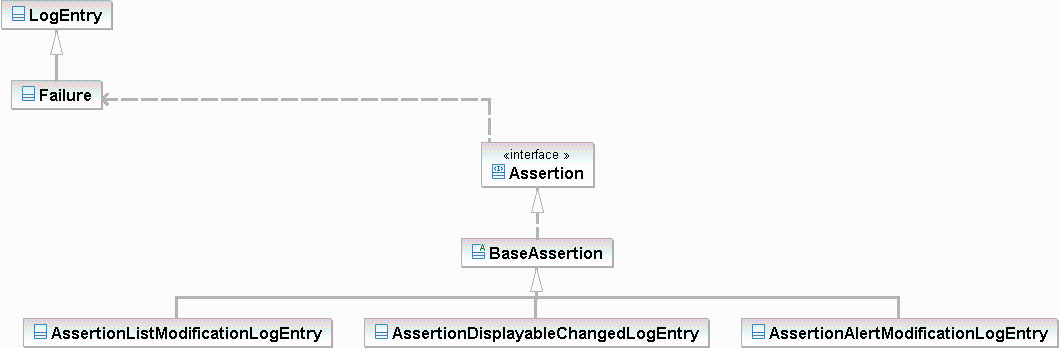
\includegraphics[width=\linewidth]{figures/uml-diagram-assertions}
\end{center}
\caption{Assertions implementation.}%
\label{fig:uml-diagram-assertions}
\end{figure}

Every time an assertion is violated a \texttt{Failure} object is created. This class is a subclass of
\texttt{LogEntry} and can be serialized to the binary protocol and transfered to the
Log Server component over a network connection. 

In the current prototype implementation of the RobotME framework there is only one action associated with
failures: terminate the whole mobile application and send every intercepted events to the
Log Server along with the Failure object itself. Then the real cause of the assertion
violations might be further investigated by the tester.

We are considering extending assertions so that there will be two types of them:
\begin{itemize}
    \item \emph{strong assertions} -- the same as in current implementation,
    \item \emph{weak assertion} -- violation of such assertion will not cause the whole mobile
  application to terminate, but only appropriate Failure object will be 
  transfered to the Log Server component. Sometimes this kind of assertions might
  be helpful with finding more errors in program execution than will be discovered
  only with strong assertions. Using this type of assertion we must be sure that after violation of
  weak assertion program will always be in consistent state, not causing
  further errors because of the weak assertion violation.
\end{itemize}
